\documentclass{standalone}
\usepackage{tikz}
\usetikzlibrary{shapes.geometric, positioning}

\begin{document}

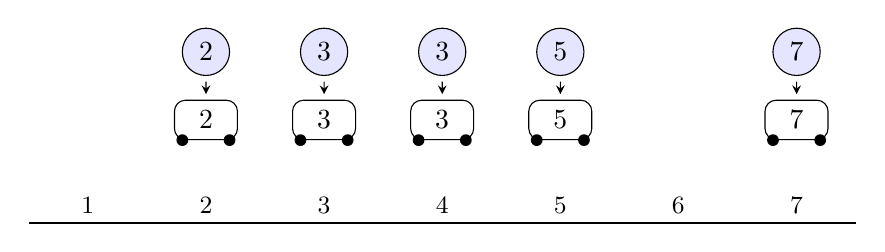
\begin{tikzpicture}[scale=1.5]

% Define styles
\tikzset{
    car/.style={draw, minimum width=0.8cm, minimum height=0.5cm, rounded corners},
    wheel/.style={circle, fill=black, inner sep=1.5pt},
    thought/.style={draw, circle, minimum size=0.6cm, fill=white!90!blue, inner sep=1pt},
    arrow/.style={->, >=stealth, shorten >=2pt, shorten <=2pt},
    label/.style={anchor=south, font=\small}
}

% Draw the parking line
\draw[thick] (-1,0) -- (6,0);
\node[label] at (-0.5,0) {1};
\node[label] at (0.5,0) {2};
\node[label] at (1.5,0) {3};
\node[label] at (2.5,0) {4};
\node[label] at (3.5,0) {5};
\node[label] at (4.5,0) {6};
\node[label] at (5.5,0) {7};

% Draw cars and thought bubbles
% Car 1
\node[car, anchor=south] (car1) at (0.5,0.7) {2};
\node[wheel] at ([shift={(-0.2,0)}]car1.south) {};
\node[wheel] at ([shift={(0.2,0)}]car1.south) {};
\node[thought, above=3mm of car1] (thought1) {2};
\draw[arrow] (thought1) -- (car1.north);

% Car 2
\node[car, anchor=south] (car2) at (1.5,0.7) {3};
\node[wheel] at ([shift={(-0.2,0)}]car2.south) {};
\node[wheel] at ([shift={(0.2,0)}]car2.south) {};
\node[thought, above=3mm of car2] (thought2) {3};
\draw[arrow] (thought2) -- (car2.north);

% Car 3
\node[car, anchor=south] (car3) at (2.5,0.7) {3};
\node[wheel] at ([shift={(-0.2,0)}]car3.south) {};
\node[wheel] at ([shift={(0.2,0)}]car3.south) {};
\node[thought, above=3mm of car3] (thought3) {3};
\draw[arrow] (thought3) -- (car3.north);

% Car 4
\node[car, anchor=south] (car4) at (3.5,0.7) {5};
\node[wheel] at ([shift={(-0.2,0)}]car4.south) {};
\node[wheel] at ([shift={(0.2,0)}]car4.south) {};
\node[thought, above=3mm of car4] (thought4) {5};
\draw[arrow] (thought4) -- (car4.north);

% Car 5
\node[car, anchor=south] (car5) at (5.5,0.7) {7};
\node[wheel] at ([shift={(-0.2,0)}]car5.south) {};
\node[wheel] at ([shift={(0.2,0)}]car5.south) {};
\node[thought, above=3mm of car5] (thought5) {7};
\draw[arrow] (thought5) -- (car5.north);

\end{tikzpicture}

\end{document}